%# -*- coding: utf-8-unix -*-
%%==================================================
%% thesis.tex
%%==================================================

\documentclass[master, fontset=windows, openright, twoside]{sjtuthesis}
% \documentclass[%
%   bachelor|master|doctor,	% 必选项
%   fontset=adobe|windows,  	% 只测试了adobe
%   oneside|twoside,		% 单面打印,双面打印(奇偶页交换页边距,默认)
%   openany|openright, 		% 可以在奇数或者偶数页开新章|只在奇数页开新章(默认)
%   zihao=-4|5,, 		% 正文字号:小四、五号(默认)
%   review,	 		% 盲审论文,隐去作者姓名、学号、导师姓名、致谢、发表论文和参与的项目
%   submit			% 定稿提交的论文,插入签名扫描版的原创性声明、授权声明 
% ]

% 逐个导入参考文献数据库
\addbibresource{bib/thesis.bib}

\begin{document}

%% 无编号内容:中英文论文封面、授权页
%# -*- coding: utf-8-unix -*-
\title{基于农业物联网和多物理场仿真的智能温室监测与控制研究}
\author{高浩天}
\advisor{黄震宇副教授}
\defenddate{2016年12月17日}
\school{上海交通大学}
\institute{电子信息与电气工程学院}
\studentnumber{1140359026}
\major{仪器仪表工程}

\englishtitle{Greenhouse Monitor}
\englishauthor{\textsc{Gao Haotian}}
\englishadvisor{Associate Prof. \textsc{Huang Zhenyu}}
\englishschool{Shanghai Jiao Tong University}
\englishinstitute{\textsc{School of Electronics and Electric Engineering} \\
  \textsc{Shanghai Jiao Tong University} \\
  \textsc{Shanghai, P.R.China}}
\englishmajor{Instrument}
\englishdate{Dec. 17th, 2016}


\maketitle

\makeenglishtitle

\makeatletter
\ifsjtu@submit\relax
	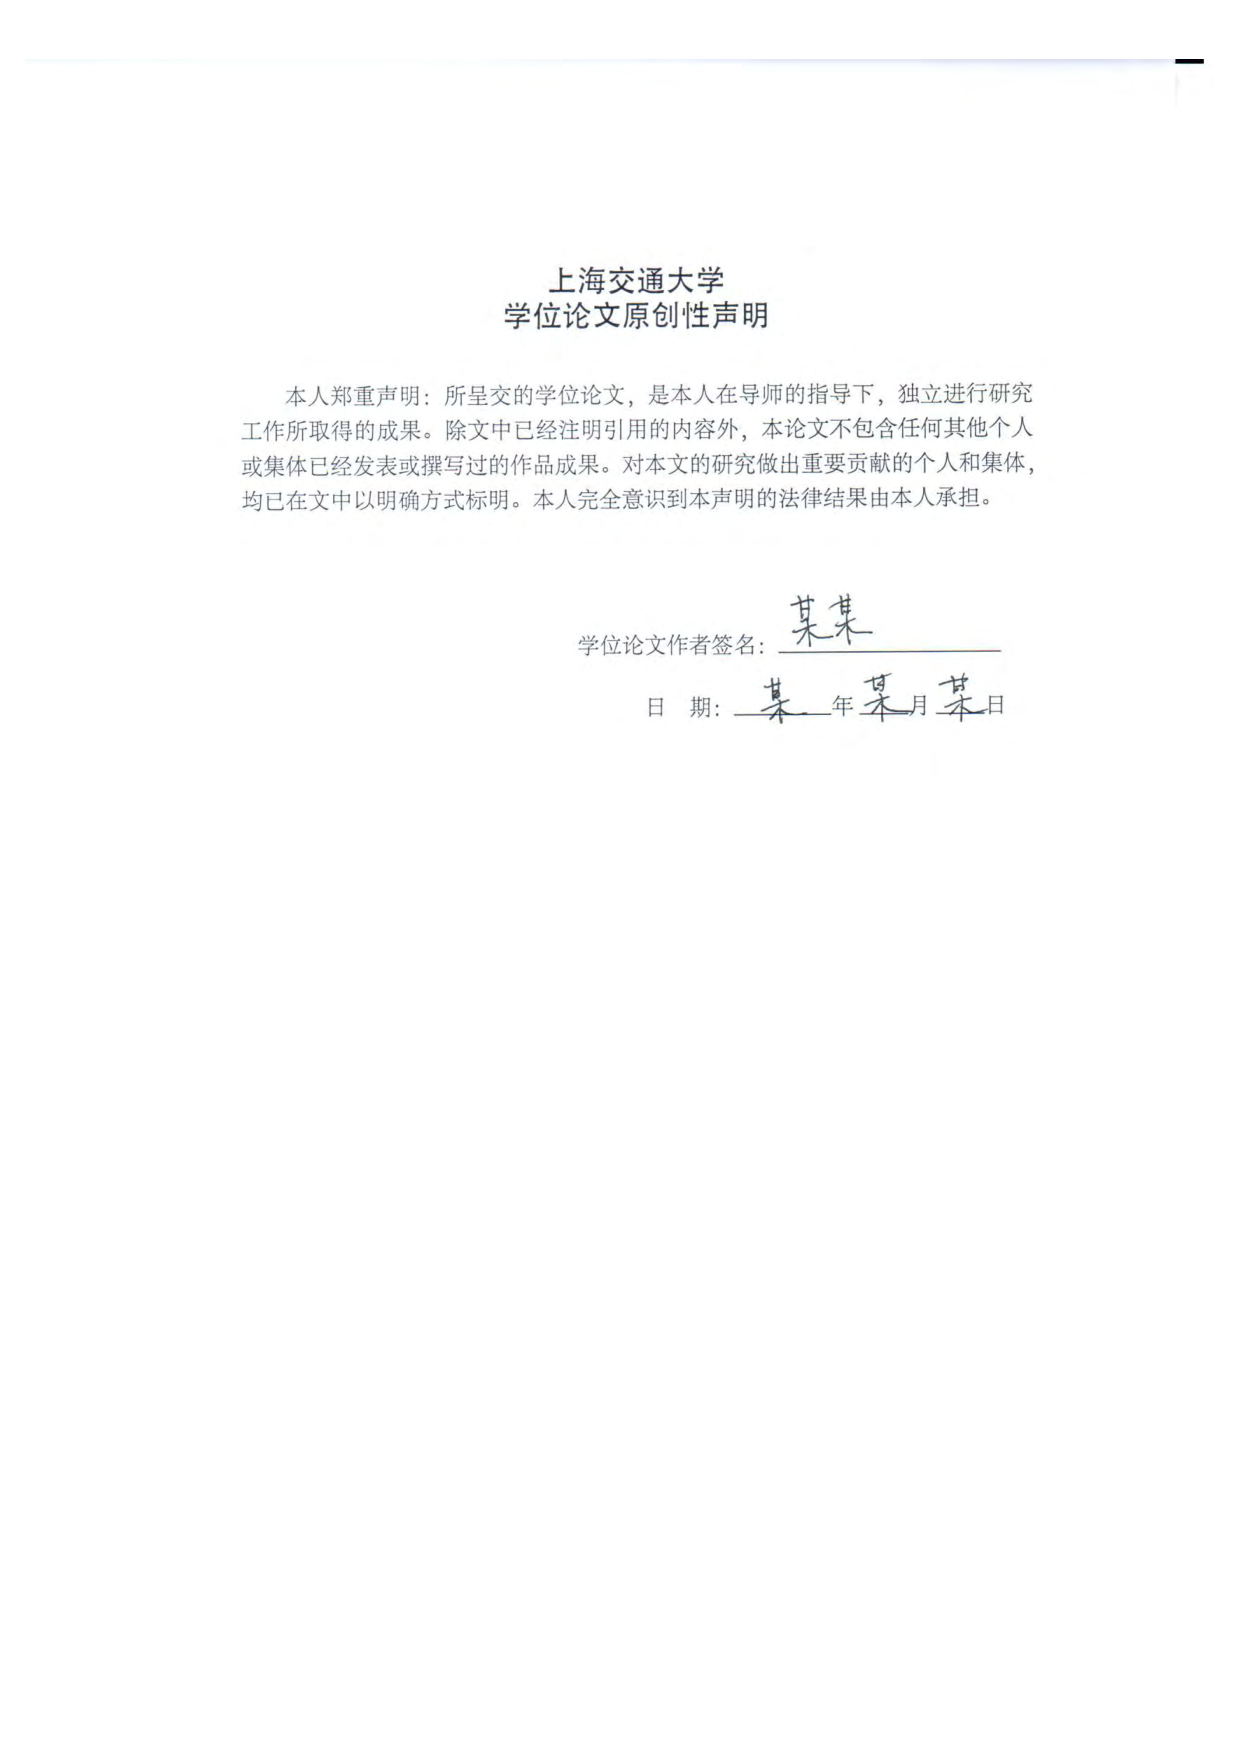
\includepdf{pdf/original.pdf}
	\cleardoublepage
	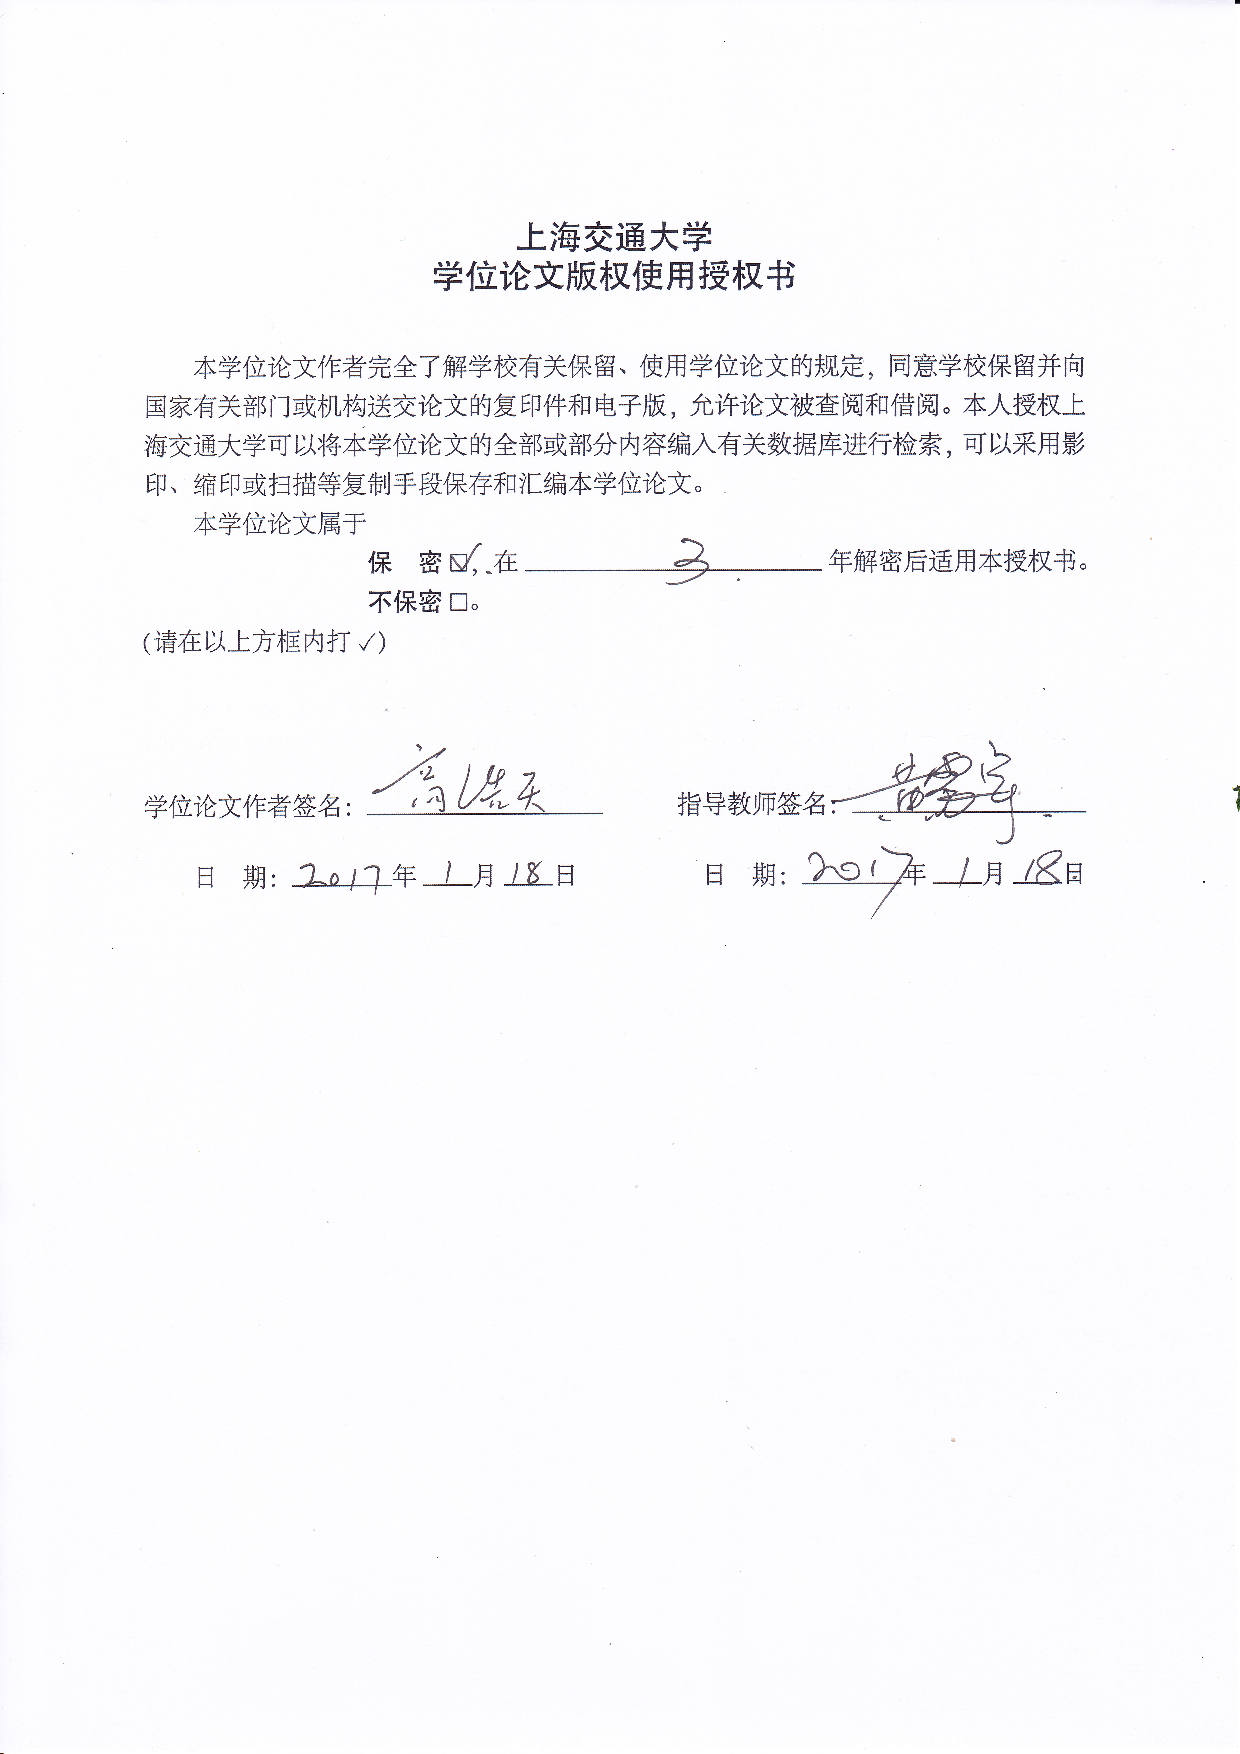
\includepdf{pdf/authorization.pdf}
	\cleardoublepage
\else
	\makeDeclareOriginal
	\makeDeclareAuthorization
\fi
\makeatother


\frontmatter 	% 使用罗马数字对前言编号

%% 摘要
\pagestyle{main}
%# -*- coding: utf-8-unix -*-
%%==================================================
%% abstract.tex for SJTU Master Thesis
%%==================================================

\begin{abstract}

农业物联网为农业生产环境的监控提供了新思路,可实现农业的智能化、信息化、精准化管理,是实现农业现代化的关键技术之一。基于农业物联网的智能温室系统,可通过网络监测温室环境,并根据作物的环境需求实施精准的温室控制,从而科学高效的管理温室。基于计算流体力学的温室仿真解决了复杂温室环境的建模分析问题,可以为智能温室系统的监测点位置优化和控制策略优化提供指导意见和理论依据。

通过分析温室监控的特殊需求并参考物联网标准架构,本文提出了基于农业物联网的智能温室架构方案。根据该架构设计了智能温室监测与控制系统:感知控制层基于ZigBee和RS485传感器网络及计算机控制模块,并针对可靠性、可扩展性、灵活性和低功耗进行了优化设计;网络传输层支持多种数据传输方式和数据同步机制,并针对网络传输的安全性、可靠性和高效性进行了重点设计,建立了系统层间枢纽;应用层包含数据中心、WEB服务器和智能策略学习控制子系统,提供了基于Hadoop和MySQL的海量温室历史数据的云存储解决方案,高可用免维护的云服务器和基于CFD仿真模型的优化控制策略;终端接入层采用WEB前端技术和React Native为系统提供了可视化界面。

智能温室监测与控制系统在实验温室进行了实测运行,运行结果表明:无线传感器网络稳定可靠,温室内外数据采集准确正常,上传同步延迟低,控制指令下达准确迅速,控制状态获取正常。数据中心工作正常,未发生慢查询或异常。云端WEB服务运行稳定,接口响应迅速,数据返回完整准确。系统满足预期设计要求和实际生产要求。

本文以南方地区典型的连栋塑料温室为研究对象,针对温室机械通风,建立了三维全尺度瞬态及稳态计算流体力学仿真模型。通过本文设计实现的智能温室监控系统,测量机械通风引起的温室内气温变化和分布,用实验验证了仿真模型瞬态和稳态计算的准确性和有效性。通过仿真模型模拟了室外高温条件下的风机数量、温室长度、入口温度及环境温度变化等参数对机械通风降温效果的影响程度,并模拟了不同数量风机启闭控制的降温效果。根据仿真分析结果优化了温室监测点位置方案和夏季机械通风控制策略。

经过对CFD仿真结果进行分析,优化后的温室监测点方案仅需最少5个监测点即可实现1280 $\text{m}^{2}$的温室整体环境状态的监测,有效减少了测点数量,降低了监测成本;优化后智能温室系统控制策略最高可减少约60\%的能源消耗,而植物冠层平均温度仅升高0.21℃,有效提高了机械通风降温效率,减少了能源消耗。

根据本文架构方案实现的智能温室监测与控制系统,节点布置灵活、监测范围广、运行功耗低、可靠性高、稳定性强、可灵活扩展,满足温室的智能和科学管理需求。结合CFD仿真分析,优化的监测点方案可有效降低监测成本,优化的机械通风控制策略可有效实现节能减排。系统还可实现异地温室集中互联,共同构建农业大数据和物联网平台,对农业科学研究和工程控制有重要意义,有助于提高农业现代化水平,推进农业物联网发展。

\keywords{\large 农业物联网 \quad 计算流体力学 \quad 温室 \quad 架构 \quad 监控系统}
\end{abstract}

\begin{englishabstract}

An imperial edict issued in 1896 by Emperor Guangxu, established Nanyang Public School in Shanghai. The normal school, school of foreign studies, middle school and a high school were established. Sheng Xuanhuai, the person responsible for proposing the idea to the emperor, became the first president and is regarded as the founder of the university.

\englishkeywords{\large SJTU, master thesis, XeTeX/LaTeX template}
\end{englishabstract}



%% 目录、插图目录、表格目录
\tableofcontents
\listoffigures
\addcontentsline{toc}{chapter}{\listfigurename} %将插图目录加入全文目录
\listoftables
\addcontentsline{toc}{chapter}{\listtablename}  %将表格目录加入全文目录
\listofalgorithms
\addcontentsline{toc}{chapter}{算法索引}        %将算法目录加入全文目录

%# -*- coding: utf-8-unix -*-
\chapter{主要符号对照表}
\label{chap:symb}

\begin{longtable}{rl}
$\epsilon$     & 介电常数 \\
 $\mu$ 		& 磁导率 \\
 $\epsilon$     & 介电常数 \\
\end{longtable}
 % 主要符号、缩略词对照表

\mainmatter	% 使用阿拉伯数字对正文编号

%% 正文内容
\pagestyle{main}
%# -*- coding: utf-8-unix -*-
%%==================================================
%% chapter0.tex for SJTU Master Thesis
%%==================================================


\chapter{绪论}
\label{chapter:Introduction}

\section{研究背景和意义}
自古以来,我们中国的祖先就知道“民以食为天”“粮食定,天下定”这一治国理政之道\supercite{ChenYunWenXuan},中国作为一个人口大国,解决全国人民的粮食食物问题是关系到国计民生的根本问题。根据农业科学院预测到2050年我国的人口将超过15亿,人口的大量增加也必然带来粮食需求量的猛增,要满足人口增长对粮食的需求,每年至少需要多生产1.2亿吨粮食。随着我国经济的飞速发展和人们生活水平的提高,人们不再仅仅关注于温饱的问题,更加追求品质生活,更加关注食品的安全、营养和多样\supercite{FengZhiming2007,ZhaoQiguo2011}。随之而来的,农业生产在不断扩大生产总量的同时也需要不断升级产业结构,以提供更加安全和高品质农副产品。

但是我国目前的农业生产的总体技术水平落后,现代化和信息化水平较低。农村的城镇化导致我国可用耕地面积不断减少,农村劳动力大量涌入城镇\supercite{YuJunli2001},务农人口急剧减少,农业生产人员逐步呈现老龄化和副业化趋势\supercite{LuoChaobin2005},传统的农业生产模式已经难以维持下去,这必然会促使农业生产者加大农药化肥产品的使用,食品安全受到前所未有的挑战,这与人民日益增长的对高品质安全食品的需求产生了难以消除的矛盾。同时随着中国市场的逐步开放,国内农产品市场与国际市场的竞争也在不断加剧。另一方面,我国还存在水资源紧缺、幅员辽阔但可用农业土地较少、生产能耗较高、基础设施建设不完善等问题。

为了解决这一系列问题,《国民经济和社会发展第十三个五年规划纲要》提出要推进农业现代化,并指出“农业是全面建成小康社会和实现现代化的基础,必须加快转变农业发展方式,着力构建现代农业产业体系、生产体系、经营体系,提高农业质量效益和竞争力,走产出高效、产品安全、资源节约、环境友好的农业现代化道路”,着重提出要推进农业物联网应用,提高农业信息化、智能化和精准化水平。

农业现代化的一个重要体现就是实现现代化的设施农业\supercite{LiuLei2013}。温室作为设施农业的重要组成部分,可以减少自然环境对于农业生产的限制,合理高效利用生产资源,人为地创造适宜的农业生产环境,提高农作物产量和质量,提高农业生产集约化程度。但是目前国内温室大多停留在电气化及以下水平,依靠农业生产者的经验对温室环境进行人工控制或电气化控制。已经实现的温室自动化监控系统多为本地监控,智能化和网络化程度较低,农业生产人员需要到现场才能获取相关数据,不便于生产应用和科学研究\supercite{duodiandapeng}。随着科技的发展进步,农业物联网为农业生产环境监控提供了新思路,通过物联网技术、传感器技术、互联网技术等先进的技术手段的综合运用可以实现农业环境的远程监测和控制,从而实现农业管理的智能化、网络化、综合化、多样化,是实现农业现代化的关键技术之一\supercite{JiYuWuLianWang,WuLianWang,ZhongGuoSheShiNongYe}。

本文课题来源于《现代农业装备与设施的研发》(沪农科攻字(2009)第8-1号),上海市2009科技兴农重点攻关项目,由上海市农业科学委员会主导并开展工作。随着今年来物联网技术、网络技术、云服务技术和智能终端的快速发展,本文综合运用物联网技术、无线传感技术和多物理场仿真技术等多领域前沿技术,设计并实现了一套基于物联网和计算流体力学仿真的智能温室监测与控制系统,该系统可远程监测和控制温室环境,让农业生产管理人员足不出户即可远程查看当前温室内的环境数据,通过视频查看当前温室内的实时情况,同时可通过远程操作温室内的作动器实现对温室内环境参数的控制。该系统还可结合种植作物的需求和当前温室内的实时环境根据智能化的温室自动控制策略实施精准的温室环境控制,从而科学高效的管理温室。消费者也可通过该系统了解到农作物的生产环境,一方面可以让消费者吃的安心放心,另一方面也可让消费者对农业生产进行监督,促进农业生产健康发展。
\section{国内外研究现状}
	\subsection{国内研究现状}
	我国是一个传统的农业大国,作为温室栽培的发源地,早在两千多年前就开始使用保护措施种植蔬菜。进入21世纪以来,我国的温室栽培技术得到快速提升,温室总面积不断增加,占据世界温室总面积的85\%以上,是温室栽培第一生产大国\supercite{WoGuoSheShiNongYe}。我国在现代温室方面的研究开始于20世纪30年代,日光温室首先在辽宁省应用于栽培蔬菜,随后我国从日本引进塑料薄膜技术开始中小拱棚的栽培,之后我国的温室一直处于发展缓慢的小规模低水平状态,直到上世纪70年代末,我国引进了一些国外的先进技术,我国的设施农业展开了新的篇章\supercite{xiandaiwenshi}。上世纪80年代开始,我国研究温室环境控制系统,并开始引入计算机控制,温室环境的控制效果得到了有效的改善\supercite{HanYi2016}。上世纪90年代后,我国在引进国外先进技术的基础上开始自主研制温室环境监控系统。上海交通大学、中国农业大学、中科院、农科院等科研院所和高校都研制出了具有不同特点的温室控制系统。
	
	经过多年的研究和时间,我国在现代温室方面的水平已经有了很大程度上的提高,但是在很多方面仍然落后于国际领先水平,主要体现在基础研究薄弱、设施结构不合理、装备和调控能力差、信息化和集约化程度低等方面\supercite{ZhangZhen2015,JiangWeijie2015} ,在温室环境的精准化、智能化控制等方面有较大的发展空间。
	\subsection{国外研究现状}
	美国、日本、荷兰等发达国家对于现代温室技术的研究起步较早,发展到今天,已经将计算机监控系统大规模应用到温室自动化生产中,在设备装备、环境控制和栽培技术等方面都处于国际领先水平。
	
	西欧是世界现代温室的发源地,虽然西欧国家的设施农业面积在世界世界设施农业总面积中占比不高,但是其现代化水平、生产质量和生产能力都非常高\supercite{GuoShirong2012}。荷兰是其中比较典型的设施农业非常发达的国家之一,主要对花卉和蔬菜进行专业化集约化生产,花卉和蔬菜出口量均居世界第一,有“欧洲菜园子”之称,其温室主要以玻璃温室为主,约占世界玻璃温室总面积的26\%以上\supercite{Watson,JiHong2007},农业生产的自动化程度很高,生产效率很高位居世界第一\supercite{QinLiu2015},其温室配套设备在满足内需的同时还大量出口到国外\supercite{Tavoletti2008Cutting}。
	
	美国的温室主要为连栋玻璃温室,现代化水平非常高。美国是最早将计算机技术投入到温室生产管理中的国家,通过政府的大力支持,采取了一系列的优惠政策,为农业现代化和信息化的发展创造了良好的氛围和环境。目前,美国约有82\%的温室采用计算机进行环境控制,27\%的农民还运用的网络技术\supercite{Kacira2011}。这样虽然提高了生产成本,但是也极大程度上给农业生产者带来了良好的经济效益\supercite{GuoShirong2012}。
	
	以色列是典型的中东国家,气候干旱,水资源匮乏,但是以色列的设施农业却非常发达,创造了沙漠中的片片绿洲,其开发的节水灌溉系统引入了计算机控制,可以精准控制水肥比例,处于世界领先水平,此外以色列对于作物生长机理的研究也比较深入,可据此建立合理的温室控制策略\supercite{GuoShirong2012,TangLibiao2003},主要生产高质量的花卉和果蔬,不仅可以自给自足还大量出口国外,享有”欧洲厨房“的美誉\supercite{QinLiu2015}。
	
	日本是一个资源非常匮乏的国家,且人口密度非常大,因此日本大力发展集约化、自动化的设施农业,主要生产果蔬和花卉,且依赖程度非常高\supercite{YangChunjun2010}。日本是最先提出植物工厂的概念,突破了土地和环境的限制,利用自动控制技术、电子技术、生物技术、机器人和新材料可以实现作物的全年连续生产,对于解决全球粮食问题和环境问题有着重要的现实意义\supercite{HuYongguang2002}。
	
	由此可见,发达国家在设施农业和现代化温室方面的研究处于非常明显的领先地位,在温室管理中大面积采用计算机控制系统,自动化和集约化程度都较高,目前正在向更为先进的智能化、精准化和网络化的方向发展。
\section{论文的主要内容与章节安排}
	\subsection{研究内容和创新点}
	本文结合物联网技术和计算力体力学仿真技术,对温室智能化监测与控制系统展开研究,主要有以下五部分内容:
		\begin{enumerate}
  			\item 适用于智能温室的农业物联网架构方案设计提出。
  			\item 针对温室机械通风三维全尺度瞬态及稳态计算流体力学仿真模型。
  			\item 针对南方地区典型的连栋塑料温室夏季机械通风实验与温室仿真模型验证。
  			\item 基于农业物联网的智能温室监测与控制系统的软件与硬件设计和实现。
  			\item 基于温室机械通风仿真模型的传感器测点位置选择与优化,及机械通风控制策略优化设计。
		\end{enumerate}
	相比于已有的相关研究,本文具有如下创新点:
		\begin{enumerate}
  			\item 本文根据农业生产环境的特殊性,通过分析温室监测与控制的特殊需求并参考物联网的标准框架,设计提出了一种适用于智能温室的农业物联网架构方案。设计并实现了基于该架构方案的智能温室远程监测与控制系统,并应用与连栋塑料温室,实现了对温室的智能感知、远程控制和智能控制,具有可靠性高、监测范围广、可灵活扩展、运行功耗低的优点,满足温室的智能运行和科学管理需求。
  			\item 为了解决我国南方地区夏季长期高温的恶劣天气对温室作物生长的严重影响,提高降温效果且减少通风能耗,本文以南方地区典型的连栋塑料温室为研究对象,针对温室机械通风,建立了三维全尺度瞬态及稳态计算流体力学仿真模型,研究了机械通风条件下温室内的气温变化和分布规律。通过在本文智能温室监测与控制系统平台上进行机械通风实验,验证了仿真模型瞬态和稳态计算的准确性和有效性。通过仿真模型模拟了室外高温条件下的风机数量、温室长度、入口温度和环境温度变化等参数对机械通风降温效果的影响程度,并模拟了不同数量风机启闭控制的降温效果,为智能温室监测和控制系统提供了优化的夏季机械通风控制策略,同时提供了优化的传感器测点布置策略,实现了以少量传感器测点数据准确反映大型温室气温分布。
		\end{enumerate}	
	\subsection{章节安排}
	本文的章节结构安排如下:
	
	第一章,绪论。介绍了本文课题的研究背景和研究意义、国内外在设施农业和现代化温室方面的研究进展和发展趋势、本文的主要研究内容和章节安排。
	
	第二章,基于农业物联网的智能温室架构。介绍物联网,提出基于农业物联网的智能温室四层架构方案,并对每层结构进行阐述和设计。
	
	第三章,智能温室监测与控制系统。详细介绍了基于本文农业物联网智能温室架构方案结合实际应用的具体实现,包括各层的硬件和软件实现。
	
	第四章,温室计算流体力学仿真及验证。基于计算流体力学建立三维全尺度瞬态及稳态机械通风仿真模型,利用本文智能温室监测与控制系统进行机械通风实验,并通过实验结果对仿真模型进行了验证。
	
	第五章,智能温室的实践与应用。详细介绍本文所设计实现的智能温室远程监测与控制系统在温室现场的实践与应用,以及温室仿真模型在实际应用中对于传感器测点位置选择优化作用和对温室机械通风控制策略的优化设计。
	
	第六章,总结与展望。总结研究内容,展望研究内容的发展前景和改进方向。

\appendix	% 使用英文字母对附录编号,重新定义附录中的公式、图图表编号样式
\renewcommand\theequation{\Alph{chapter}--\arabic{equation}}	
\renewcommand\thefigure{\Alph{chapter}--\arabic{figure}}
\renewcommand\thetable{\Alph{chapter}--\arabic{table}}
\renewcommand\thealgorithm{\Alph{chapter}--\arabic{algorithm}}

%% 附录内容,本科学位论文可以用翻译的文献替代。
%# -*- coding: utf-8-unix -*-
%% app2.tex for SJTU Master Thesis
%% based on CASthesis
%% modified by wei.jianwen@gmail.com
%% version: 0.3a
%% Encoding: UTF-8
%% last update: Dec 5th, 2010
%%==================================================

\chapter{Maxwell Equations}

选择二维情况,有如下的偏振矢量:
\begin{subequations}
  \begin{eqnarray}
    {\bf E}&=&E_z(r,\theta)\hat{\bf z} \\
    {\bf H}&=&H_r(r,\theta))\hat{ \bf r}+H_\theta(r,\theta)\hat{\bm
      \theta}
  \end{eqnarray}
\end{subequations}
对上式求旋度:
\begin{subequations}
  \begin{eqnarray}
    \nabla\times{\bf E}&=&\frac{1}{r}\frac{\partial E_z}{\partial\theta}{\hat{\bf r}}-\frac{\partial E_z}{\partial r}{\hat{\bm\theta}}\\
    \nabla\times{\bf H}&=&\left[\frac{1}{r}\frac{\partial}{\partial
        r}(rH_\theta)-\frac{1}{r}\frac{\partial
        H_r}{\partial\theta}\right]{\hat{\bf z}}
  \end{eqnarray}
\end{subequations}
因为在柱坐标系下,$\overline{\overline\mu}$是对角的,所以Maxwell方程组中电场$\bf E$的旋度:
\begin{subequations}
  \begin{eqnarray}
    &&\nabla\times{\bf E}=\mathbf{i}\omega{\bf B} \\
    &&\frac{1}{r}\frac{\partial E_z}{\partial\theta}{\hat{\bf
        r}}-\frac{\partial E_z}{\partial
      r}{\hat{\bm\theta}}=\mathbf{i}\omega\mu_rH_r{\hat{\bf r}}+\mathbf{i}\omega\mu_\theta
    H_\theta{\hat{\bm\theta}}
  \end{eqnarray}
\end{subequations}
所以$\bf H$的各个分量可以写为:
\begin{subequations}
  \begin{eqnarray}
    H_r=\frac{1}{\mathbf{i}\omega\mu_r}\frac{1}{r}\frac{\partial
      E_z}{\partial\theta } \\
    H_\theta=-\frac{1}{\mathbf{i}\omega\mu_\theta}\frac{\partial E_z}{\partial r}
  \end{eqnarray}
\end{subequations}
同样地,在柱坐标系下,$\overline{\overline\epsilon}$是对角的,所以Maxwell方程组中磁场$\bf H$的旋度:
\begin{subequations}
  \begin{eqnarray}
    &&\nabla\times{\bf H}=-\mathbf{i}\omega{\bf D}\\
    &&\left[\frac{1}{r}\frac{\partial}{\partial
        r}(rH_\theta)-\frac{1}{r}\frac{\partial
        H_r}{\partial\theta}\right]{\hat{\bf
        z}}=-\mathbf{i}\omega{\overline{\overline\epsilon}}{\bf
      E}=-\mathbf{i}\omega\epsilon_zE_z{\hat{\bf z}} \\
    &&\frac{1}{r}\frac{\partial}{\partial
      r}(rH_\theta)-\frac{1}{r}\frac{\partial
      H_r}{\partial\theta}=-\mathbf{i}\omega\epsilon_zE_z
  \end{eqnarray}
\end{subequations}
由此我们可以得到关于$E_z$的波函数方程:
\begin{eqnarray}
  \frac{1}{\mu_\theta\epsilon_z}\frac{1}{r}\frac{\partial}{\partial r}
  \left(r\frac{\partial E_z}{\partial r}\right)+
  \frac{1}{\mu_r\epsilon_z}\frac{1}{r^2}\frac{\partial^2E_z}{\partial\theta^2}
  +\omega^2 E_z=0
\end{eqnarray}


\backmatter	% 文后无编号部分 

%% 参考资料
\printbibliography[heading=bibintoc]

%% 致谢、发表论文、申请专利、参与项目、简历
%% 用于盲审的论文需隐去致谢、发表论文、申请专利、参与的项目
\makeatletter

%%
% "研究生学位论文送盲审印刷格式的统一要求"
% http://www.gs.sjtu.edu.cn/inform/3/2015/20151120_123928_738.htm

% 盲审删去删去致谢页
\ifsjtu@review\relax\else
  %# -*- coding: utf-8-unix -*-
\begin{thanks}

提笔写下这段致谢辞,才惊觉自己即将真正离开,人生亦从此开始新的篇章。尽管不舍,却更珍惜,因为我的生命中有那么多可爱的人值得感激。他们使我的大学生活充满了色彩,无论收获、遗憾,对我来说都是值得珍藏的记忆。“享其实者思其树,饮其流者怀其源,学其成者念吾师”,在此论文完成之际,谨向我尊敬的指导老师黄震宇老师致以诚挚的谢意和崇高的敬意。黄老师不仅在学业上言传身教,而且以其高尚的品格给我以情操上的熏陶。本文的写作更是直接得益于他的悉心指点,从论文的选题到体系的安排,字句的斟酌,无不凝聚着他的心血。师恩重于山,无法用言语形容感激,惟愿师生情谊一生延续。在此还要感谢符凌峰,朱森林,常歌等师兄师弟在系统硬件上给予我无私的帮助,帮助我顺利的完成硕士课题。

感谢上海交通大学对我的培养,学校的培养让我学到了专业的科学文化知识,同时也提升了我的多方面的能力,塑造了我的人格,使我在未来的人生道路上能够更加信心百倍的走下去。
感谢我的父母,我的家人。焉得谖草,言树之背,养育之恩,无以回报。你们始终如一的支持和关爱是我人生道路不断前进的强大动力,教我学会坚强、勇敢,使我在磨砺中得到成长。祝你们永远健康快乐,这是我最大的心愿和牵挂。

在此,祝老师同学们,以及所有关心我的人和我所关心的人身体健康,工作顺利,心情愉快,幸福平安!
\end{thanks}
 	  %% 致谢
\fi

  % 盲审论文中,发表学术论文及参与科研情况等仅以第几作者注明即可,不要出现作者或他人姓名
\ifsjtu@review\relax
  %# -*- coding: utf-8-unix -*-

\begin{publications}{99}
    \item\textsc{第一作者}. {中文核心期刊论文}, 2007.  
    \item\textsc{第一作者}. {EI国际会议论文}, 2006.
\end{publications}

  %# -*- coding: utf-8-unix -*-

\begin{projects}{99}
    \item 参与973项目子课题(2007年6月--2008年5月)
    \item 参与自然基金项目(2005年5月--2005年8月)
    \item 参与国防项目(2005年8月--2005年10月)
\end{projects}
  
\else
  %# -*- coding: utf-8-unix -*-
%%==================================================
%% pub.tex for SJTUThesis
%% Encoding: UTF-8
%%==================================================

\begin{publications}{99}
    \item\textsc{黄震宇, 高浩天, 朱森林, 赵春宇, 蔡春花}. {南方连栋塑料温室夏季机械通风优化设计}[J]. 农业机械学报, 已录用.
    \item\textsc{高浩天, 朱森林, 常歌, 符凌峰, 黄震宇}. {基于农业物联网的智能温室系统架构与实现}[J]. 农机化研究, 已录用.
    \item\textsc{李腾, 高浩天, 赵春宇, 朱成刚, 黄震宇}. {种子风力筛选机分离室内气固两相流仿真与优化}[J]. 农机化研究, 2016,07:85-89.
    \item\textsc{符凌峰, 赵春宇, 黄震宇, 高浩天}. {基于ZigBee技术的连栋温室低功耗环境监测系统设计}[J]. 传感器与微系统, 2016, 08:74-76+79.
\end{publications}
	      %% 发表论文
  %# -*- coding: utf-8-unix -*-
%%==================================================
%% projects.tex for SJTUThesis
%% Encoding: UTF-8
%%==================================================

\begin{projects}{99}
    \item 973项目“XXX”
    \item 自然基金项目“XXX”
    \item 国防项目“XXX”
\end{projects}
  %% 参与的项目
\fi

% %# -*- coding: utf-8-unix -*-
\begin{patents}{99}
    \item 第一发明人,“永动机”,专利申请号202510149890.0
\end{patents}
	  %% 申请专利
% \include{tex/resume}	  %% 个人简历

\makeatother

\end{document}
